\documentclass{article}

\usepackage{tikz}

\begin{document}
\title{Quantum computer architecture}
 \author{John Scott, Oliver Thomas}
\maketitle

\abstract{This is for a demonstration of 12 or 16 \textit{Classical qubits} to
    demonstrate the differences between a 4 bit digital microcomputer and state of the
art quantum processors}

\section{Notes about the electronic design}

\begin{itemize}
    \item 16 qubits (4 by 4 grid) requires $2^{16}=65536$ entries in the state vector. Each entry must be signed and could optionally be complex (to express the addition algorithm). If we used 4 bits of precision that means complex amplitudes require 16bits. Then the state vector can be stored in 131072 Bytes (approx. 131 KiB).

\item Multiplication requires only 2 by 2 and 4 by 4 matrix multiplications. The unitary operations can be performed in block diagonal form. You probably need 2 or 3 external memory chips (one for the state vector and a few for working memory).

\item States of qubits will be shown using RGB LEDs. We also need to figure out how to measure.

\item The memory needs to be quite fast. We found one (AS6C4008-55PCN) that has 55ns
    read/write times (we think). The time it takes the micro-controller to do the matrix
    multiplication is also important. If the micro-controller has 70MHz instruction rate
    and a single matrix multiplication takes 200 clock cycles for a 4 by 4 matrix (guess)
    then the total processing will take about 40ms assuming that you need to do $2^{14}$ blocks. That seems quick enough.
  
\item We could cycle between the non-zero amplitudes to show the super-position. If you
    did it fast enough in proportion to different amplitude sizes it would do the
    averaging for you.
\end{itemize}

\section{Notes about aesthetics/interface}
\begin{itemize}
\item Grid of 4 by 4 LEDs with colors showing qubit state.
\item We will use buttons to perform the gates. For two qubit gates: We can have buttons placed between the LEDs (connecting each qubit), and a control panel at the bottom for each different kind of gate (CNOT, CPhase, etc.). The user presses one of each to perform a particular gate between two qubits. For one qubit gates: We can have buttons on each qubit (on the display area) to select a qubit and then use buttons on the control panel to select the one qubit gate (X, H, etc.) We could use flashing to indicate when a qubit is selected. We could even just have buttons on the qubits only, and perform two qubit gates by pressing one after the other.
\item Mechanical back-lit switches are the only way!
\end{itemize}

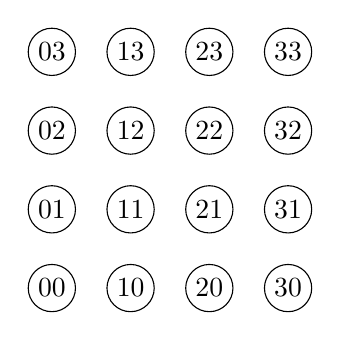
\begin{tikzpicture}
\centering
    \foreach \x in {0,...,3}
    \foreach \y in {0,...,3}
    \draw (\x,\y) circle (0.3) node {\x\y};

\end{tikzpicture}

\end{document}
